\documentclass[11pt,a4paper]{report}
\usepackage[utf8]{inputenc}
\usepackage[portuges]{babel}
\usepackage{graphicx}
\newcommand*{\escape}[1]{\texttt{\textbackslash#1}}
\usepackage{etoolbox}% http://ctan.org/pkg/etoolbox
\makeatletter
% \patchcmd{<cmd>}{<search>}{<replace>}{<success>}{<failure>}
% --- Patch \chapter
\patchcmd{\@makechapterhead}{50\p@}{\chapheadtopskip}{}{}% Space from top of page to CHAPTER X
\patchcmd{\@makechapterhead}{12\p@}{\chapheadsep}{}{}% Space between CHAPTER X and CHAPTER TITLE
\patchcmd{\@makechapterhead}{40\p@}{\chapheadbelowskip}{}{}% Space between CHAPTER TITLE and text
% --- Patch \chapter*
\patchcmd{\@makeschapterhead}{50\p@}{\chapheadtopskip}{}{}% Space from top of page to CHAPTER TITLE
\patchcmd{\@makeschapterhead}{40\p@}{\chapheadbelowskip}{}{}% SPace between CHAPTER TITLE and text
\makeatother
% Set new lengths
\newlength{\chapheadtopskip}\setlength{\chapheadtopskip}{20pt}
\newlength{\chapheadsep}\setlength{\chapheadsep}{40pt}
\newlength{\chapheadbelowskip}\setlength{\chapheadbelowskip}{15pt}

\title{Processamento de Linguagens (3º ano de Curso)\\
       \textbf{Trabalho Prático 2}\\ Relatório de Desenvolvimento
       } %Titulo do documento
%\title{Um Exemplo de Artigo em \LaTeX}
\author{Joana Cruz\\ (A76270) \and Maurício Salgado\\ (A71407)
         \and Rui Azevedo\\ (A80789)
       } %autores do documento
\date{\today}

\begin{document}

\maketitle

\newpage

\begin{abstract}
    \qquad O presente trabalho tem como objectivo aumentar a experiência de uso do ambiente \textit{Linux} e de algumas ferramentas de apoio à programação, aumentar a capacidade de escrever \textit{Expressões Regulares (ER)} para a descrição de padrões de frase, desenvolver sistemática e automaticamente processadores de linguagens regulares que filtrem  ou transformem textos e utilizar o sistema de produção para filtragem de texto \textbf{\textit{GAWK}}.
\end{abstract}

\tableofcontents

\chapter{Introdução}

\section{Preliminares}
    \qquad O objectivo deste relatório é demonstrar o processo de desenvolvimento de um processador de ficheiros, capaz de extrair um conjunto de informações de acordo com os requisitos estabelecidos. Para este efeito, desenvolveu-se um conjunto de \textit{scripts} utilizando o sistema de produção para filtragem de texto, \textbf{\textit{GAWK}}, de modo analisar e extrair um conjunto de dados de um ficheiro.
    
    \quad O ficheiro a processar contém informação sobre uma colecção de cartas trocadas nos anos de mil e seiscentos aquando da viagem dos navegadores portugueses à Etiópia.
    
\section{Enunciado do trabalho e objetivos}
    \qquad Analise com todo o cuidado o ficheiro \textbf{\textit{natura.di.uminho.pt/~jj/pl-19/TP2/cartasetiopia.csv}} o qual contém informação diversa sobre uma colecção de cartas trocadas nos anos de mil seiscentos aquando da viagem dos navegadores portuguesas à Etiópia.

    \qquad Construa então um ou mais programas \textit{\textbf{AWK}} que processem esse arquivo de modo a:
    
    \begin{itemize}
        \item contar o número de cartas por local, relacionando-as com o ano de escrita.
        \item criar um \textit{index} \textbf{HTML} com todos os anos, em que cada ano deve ligar a outra página HTML onde conste, para cada carta desse ano, o título da carta e o seu resumo.
        \item mostrar a lista das cartas — cada uma identficada pelo número, devidamente associada (em pares número-nome) aos apelidos das pessoas envolvidas no assunto relatado.
        \item desenhar um grafo (em \textbf{\textit{DOT})} que relacione cada autor (identificado pelo seu nome) com o destinatário (também identificado pelo nome).
    \end{itemize}

\section{Estrutura do relatório}

    \qquad O presente relatório visa apresentar os diferentes passos tomados na conceção de um conjunto de programas que filtram e extraem um conjunto de informações de um ficheiro.
    
    \quad Irá ser contextualizado o problema em questão bem como os objetivos com a realização deste trabalho.
    
    \quad De seguida, apresentámos as características dos dados e decisões tomadas durante o desenvolvimento do projeto. 
    
    \quad Por fim iremos apresentar e analisar os diferentes \textit{scripts} desenvolvidos para responder aos requisitos pedidos, apresentando também um excerto do ficheiro a processar bem como os resultados obtidos após a execução desses \textit{scripts}.
\\
\\
\section{Características dos dados e decisões}
    \qquad O ficheiro a processar tem o formato de um \textit{Comma-Separated-Values (CSV)}. Este tipo de ficheiros armazenam informação em forma tabular em \textit{plain text}, sendo que cada linha do ficheiro representa um registo que contém um ou mais campos.
    
    \qquad Uma vez que o ficheiro já vem formatado de uma maneira conveniente, o processo de criação de filtros torna-se mais fácil.
    
    \qquad Neste ficheiro, cada registo apresenta informação relativa a uma carta. De seguida apresentámos a estrutura de um registo de uma carta:
\\

\begin{table}[h]\centering
    \begin{tabular}{|c|c|c|c|c|c|c|}
    \hline
    \textbf{\$1} & \textbf{\$2} & \textbf{\$3} & \textbf{\$4} & \textbf{\$5} & \textbf{\$(\textgreater{}=6)} & \textbf{} \\ \hline
    ID           & Data         & Local        & Informacao   & Apelidos     & Resumo                     & ...       \\ \hline
    \end{tabular}
    \caption{Campos do registo de uma carta}
\end{table}

\quad Os seis primeiros campos são fixos, ou seja, uma carta tem sempre a informação apresentada na tabela. No entanto, o resumo da carta pode estar repartido por diferentes campos. 
%% Implementacao -----------------------------

\chapter{Implementação}
\qquad Neste capítulo iremos apresentar os padrões criados em \textbf{\textit{GAWK}} de modo a responder aos requisitos estabelecidos. Foram criados, para este fim, quatro ficheiros, cada um contendo um conjunto de padrões que resolvem um requisito.

\section{Número de cartas por local}

\qquad O seguinte \textit{script} apresenta um conjunto de filtros que permitem apresentar informação relativa ao número de cartas escritas no determinado local, sendo que estas cartas são relativas a uma data de criação.

\quad Numa primeira fase, definimos o carácter \textbf{";"} como o separador de filtros e o carácter \textbf{"\escape{n}"} como o separador de registos (separador de registos por omissão). De seguida, normalizamos os campos dos diferentes registos, limpando os espaços em branco através da função pré-definida do \textbf{\textit{GAWK}}, \textbf{\textit{gsub}}. Como alguns registos de cartas não apresentam informação relativa ao local de emissão, este campo nesses registos foi alterado para a \textit{string \textbf{NIL}}. 

\quad Após a normalização dos diferentes campos dos registos, foi criada a estrutura de dados \textit{nr\_cartas} que vai guardar a correspondência entre um local, uma data e respetivos números de cartas. 

\quad De seguida apresentámos duas instâncias desta estrutura.
\small{
\begin{verbatim}
    nr_cartas["Etiópia"]["1626.06.01"] == 2
    nr_cartas["Goa"]["1652.10.16"] == 1
    ...
\end{verbatim}

\quad Por último, no fim de percorrer todos os registos, os resultados da filtragem do ficheiro são impressos no seguinte formato:

\begin{verbatim}
    > Local
            Data1       nr_cartas
            Data2       nr_cartas
            ...         ...
            ---------------------
            Total =     total_cartas_local
\end{verbatim}

De seguida apresentámos o \textit{script} desenvolvido para obter a informação pedida.

\newpage

\begin{verbatim}
##############################################
#
# Definicao do Field Separator
# RS = \n (por omissao)
#
##############################################
BEGIN {FS=";"}
##############################################
#
# Normalizacao de todos os campos do registo
#
##############################################
{ 
for(i = 1; i <= NF; i++) 
    gsub(/^\s+|[]]|\s+$|\s+(?=\s)/,"",$i)
}
##############################################
#
# Se nao existir local coloca o campo com o
# valor de NIL
#
##############################################
length($3)==0	{$3 = "NIL"}
##############################################
#
# Estrutura que armazena o numero de cartas 
# por local relacionando com o ano de escrita
#
##############################################
NF>5		{nr_cartas[$3][$2]++}
##############################################
#
# No fim de percorrer todos os registos e
# impresso o resultado
#
##############################################
END{
    for(i in nr_cartas){
        printf("> %s\n",i)
        for(j in nr_cartas[i]){
            total += nr_cartas[i][j]
            printf("\t %4s %6s\n",j, nr_cartas[i][j])
        }
	    printf("         %s\n","-----------------")
	    printf("\t %4s =    %6s\n\n","Total",total)
	    total = 0
    }
}
\end{verbatim}}


\section{Gerar ficheiros \textit{HTML}}

\quad O objetivo deste requisito é criar um índice \textit{\textbf{HTML}} com os anos de todas as cartas contidas no ficheiro. Esses índices ligam a outras páginas \textbf{\textit{HTML}} onde constam, para cada carta desse ano, o título da carta e o seu resumo.

\quad Em primeiro lugar, antes do processamento dos registos, foram definidos o separador de registo e de campos. Para além disso, foram definidas as \textit{tags} necessárias para criar o ficheiro \textbf{\textit{HTML}} e gravadas no ficheiro \textit{index.html}.

\quad De seguida, procedeu-se à normalização dos campos dos diferentes registos, limpando os espaços em branco e partindo a data de modo a termos somente o campo relativo ao ano da carta. Para além disso, uma vez que o resumo da carta está repartido por vários campos de um registo, foi feita a concatenação destes campos de modo a termos uma única \textit{string} que contenha essa informação.

\quad Após a normalização dos registos, a correspondência \textit{ano -> título -> resumo} é armazenada numa estrutura de dados \textit{anos}. De seguida apresentámos um exemplo dessa estrutura:

\begin{verbatim}
    ano[Ano][Titulo] = Resumo
\end{verbatim}

\quad Por fim, ao fim do processamento de todos os registos, e já com a estrutura devidamente preenchida, essa informação é disposta nas respetivas nas devidas páginas \textbf{\textit{HTML}} guardando essa informação no ficheiro \textit{index.hmtl}.

\quad De seguida, é apresentado o \textit{script} desenvolvido para gerar os diversos ficheiro \textbf{\textit{HTML}}.
\\
\\
\begin{verbatim}
##############################################
#
# Definicao do Field Separator
# RS = \n (por omissao)
#
# Definicao de tags HTML
#
##############################################

BEGIN { FS=";"
headerTitle="Processamento de Linguagens-TP2";
bodyTitle="Índice de anos";
headerFormat= "<html><head><meta charset = 'UTF-8'/><title>%s</title></head><body><center>
               <h1>%s</h1></center><ul>\n";
refHtml = "<a href=file:///Users/ruiazevedo/Desktop/Universidade/PL/PL/Fase2/%s>%s</a>\n";
textHtml = "<h3>%s</h3>%s";
endHtml = "</ul></body></html>";
printf headerFormat , headerTitle , bodyTitle > "index.html";
}
\end{verbatim}
\newpage
\begin{verbatim}
##############################################
#
# Normalizacao de todos os campos do registo
#
# No campo $2 (datas), apenas nos interessa 
# o ano
#
##############################################
{ 	
for(i = 1; i <= NF; i++) 
    gsub(/^\s+|\s+$|\s+(?=\s)/,"",$i)
gsub(/\.[0-9.]+/,"",$2);
}
##############################################
#
# Agregacao de todos os campos a partir do
# campo $6 numa unica string
#
# Estes campos representao a descricao da carta
# dai necessitarmos de os agregar
#
# Estrutura 'ano' que armazena a correspondencia
# entre uma data um titulo de uma carta e a 
# respetiva descricao
#
##############################################
{
for(i=6; i <=NF; i++)
    str=sprintf("%s %s", str, $i);
ano[$2][$4] = str;
str = NULL;
}
##############################################
#
# No fim de percorrer todos os registos são
# gerados os ficheiros HTML
#
##############################################

END {  	
    for(i in ano){
	        printf headerFormat, headerTitle, i > i".html";
            for(j in ano[i])
                printf textHtml, j, ano[i][j] > i".html";
            printf endHtml > i".html";
            printf refHtml, i".html", i > "index.html";
        }
        print endHtml > "index.html"; 
}



\end{verbatim}

\section{Lista de cartas}

\quad O objetivo pretendido deste requisito é apresentar a lista de cartas, cada uma associada aos apelidos das pessoas envolvidas no assunto relatado. 

\quad Mais uma vez, o primeiro passo é definir os separadores de registo e de campos, seguido da normalização desses mesmos campos.

\quad A informação relativa aos apelidos das pessoas envolvidas no assunto da carta está presente no campo 5 dos registos. Dado que cada um desses campos contém mais que um apelido, é necessário partir esse campo em \textit{n} partes, sendo \textit{n} o número de apelidos presentes nesse campo. A função pré-definida \textit{split} permite com que seja possível partir um campo de um registo em várias \textit{strings}, definindo um separador de campos. O formato do campo 5 dos registo é do tipo:

\begin{verbatim}
    $5 := "     GOA :        AZEVEDO :      FILIPE III :"
\end{verbatim}

Para a \textit{string} ser partida em apelidos, desenvolveu-se uma expressão regular que encontra nomes numa string, ignorando espaços em branco insignificantes. Essa expressão pode ser definida da seguinte maneira:

\begin{verbatim}
    regexp(Apelidos) := "\s{2,}|:"
\end{verbatim}

\quad Uma vez feita a sua normalização, os dados são impressos com a seguinte estrutura :

\begin{verbatim}
    Número da carta : <nr_carta>
    Apelidos : <lista_apelidos>
\end{verbatim}

\quad De seguida, apresentámos o \textit{script} desenvolvido para gerar a informação pedida.

\newpage 
\begin{verbatim}
##############################################
#
# Definicao do Field Separator
# RS = \n (por omissao)
#
##############################################

BEGIN {FS=";"}
\end{verbatim}

\begin{verbatim}

##############################################
#
# Normalizacao de todos os campos do registo 
#
##############################################

{
for(i = 1; i <= NF; i++)
	if(i != 5 )
      	gsub(/^\s+|\s+$|\s+(?=\s)/,"",$i)
}

##############################################
#
# Parte o campo $5 em apelidos através da 
# funcao split. Em cada posicao do array
# apelidos temos um apelido
#
##############################################

{split($5,apelidos,/\s{2,}|:/)}
#{split($5,apelidos,/[^a-zA-ZáÁéÉóÓçÇ]+/)}

##############################################
#
# Imprime o resultado ao fim de processar 
# cada record
#	result := <id,[Apelidos]>
#
##############################################

length(apelidos)>0	   { printf("Número da carta: %d\n",$1);	
					printf("Apelidos: ")
					
					for(i in apelidos) 
						if(length(apelidos[i])>0)
							printf("%s| ", apelidos[i])
					print "\n" 
					}

\end{verbatim}

\section{Grafo \textit{DOT}}

\qquad É pretendido, neste requisito, que seja gerado um ficheiro \textbf{\textit{DOT}} de maneira a gerar um grafo que relacione cada autores com o destinatário das cartas.

\quad O formato do \textit{script} a criar é o seguinte:

\begin{verbatim}
    diagraph grafo{
        Autor -> Destinatário;
        ...
    }
\end{verbatim}

\quad O primeiro passo é sempre normalizar os diferentes campos do registo e definir os devidos separadores. Para além disso, é inicializada a estrutura de um grafo em notação \textbf{\textit{DOT}} escrevendo-a no ficheiro \textit{graph.gv}.

\quad Após a normalização dos dados, é necessário recolher a informação dos diferentes autores e destinatários. Para isto, analisamos o campo 4 dos diferentes registos de modo a encontrar um padrão que nos permita descobrir os autores e destinatários. Após esta análise, podemos verificar que os seguintes padrões: 

\begin{verbatim}
    (1) Carta <preposição> <nome> <preposição> <nome>
    (2) Certidão da carta <preposição> <nome> <preposição> <nome>
    (3) Requerimento <preposição> <nome> <preposição> <nome>
    
        <preposição> := de || do || a || ao || aos 
    
\end{verbatim}

\quad De modo a obter os autores e destinatários corretamente, vamos filtrar todos os registos cujo o campo 4 contém as palavras Carta, Requerimento ou Certidão. Após feita a correspondência apagámos essas palavras do registo ficando apenas com informação no formato: 

\begin{verbatim}
    <nome> <preposição <nome>
    
        <preposição> := a || ao || aos
\end{verbatim}

Existem alguns casos particulares no ficheiro de input em que o autor ou o destinatário são anónimos que também foram corretamente processados:
\begin{verbatim}
    (1) Carta <ao> <nome>
    (2) Carta <preposição> <nome>
    (1) Certidão da carta <pelo> <nome>
    
        <preposição> := de || do
\end{verbatim}
\quad De seguida, partimos essa \textit{string} através da função pré-definida \textit{split}, sendo o separador de campo as diferentes preposições definidas. Após esta filtragem, é escrito no ficheiro \textit{graph.gv} a seguinte \textit{string}:

\begin{verbatim}
    Autor -> Destinatário;
\end{verbatim}

\quad Ao fim de processar todos os registos, fechámos a definição da estrutura do grafo escrevendo no ficheiro o carácter \textbf{\textit{\}}}.

\quad De seguida, apresentámos o \textit{script} criado para gerar o ficheiro em formato \textbf{\textit{DOT}}.
\newpage 
\small{
\begin{verbatim}
##############################################
# Definicao do Filter Separator
# RS = \n (por omissao)
#
# Inicio da estrutura de dados de um grafo
#
#	digraph grafo {
#		size="100,100";
#
# Escrita do inicio da estrutura no ficheiro
# graph.gv
##############################################
BEGIN { FS=";"
        graph = "digraph grafo {\n\tsize=\"100,100\";\n\trankdir=LR;\n";
        printf graph > "graph.gv";}
##############################################
# Normalizacao de todos os campos do registo
##############################################
{ 	
for(i = 1; i <= NF; i++) 
    gsub(/^\s+|\s+$|\s+(?=\s)/,"",$i)
}
##############################################
# Encontra todas as linhas cujo campo $4 (Titulo)  
# contenha a palavra carta, requerimento ou 
# certidao 
# Parte-se a frase na proposicao 'ao' e guarda
# no array 'autores' o resultado
#   autores[1] := Autor
#   autores[2] := Destinatario
#
# Adiciona ao ficheiro graph.gv sd relacoes
#	"autor" -> "destinatario";
##############################################
$4 ~ /(Carta|Requerimento|Certidão)/ 
{	
    gsub(/((Carta|Requerimento|Certidão)(([^iA-Z]+)(d(e|o)+|pelo) | enviada|)|>.+)/,"",$4);
    split($4,autores,/ ao?s? /)
					
    if( contain[autores[1]][autores[2]] == 0 ){
        autor = "\t\"%s\" -> \"%s\";\n";
        printf autor, autores[1], autores[2] > "graph.gv";
        contain[autores[1]][autores[2]]++
}
##############################################
# No fim de percorrer todos os registos fecha
# a definicao da estrutura do grafo
##############################################
END { printf "}" > "graph.gv";}
\end{verbatim}}

\chapter{Apresentação de resultados}
\section{Input}

\qquad Nesta secção apresentámos um excerto do conteúdo do ficheiro a processar que contém apenas 17 registos. O ficheiro original contém 67 linhas, logo 67 registos, cada um com o número de campos variável.

\qquad Podemos verificar, como já foi referido, que o ficheiro está organizado de forma tabular, um registo por linha e um conjunto de campos por registo separados pelo carácter \textbf{;}
\\
\\
\begin{figure}[h]
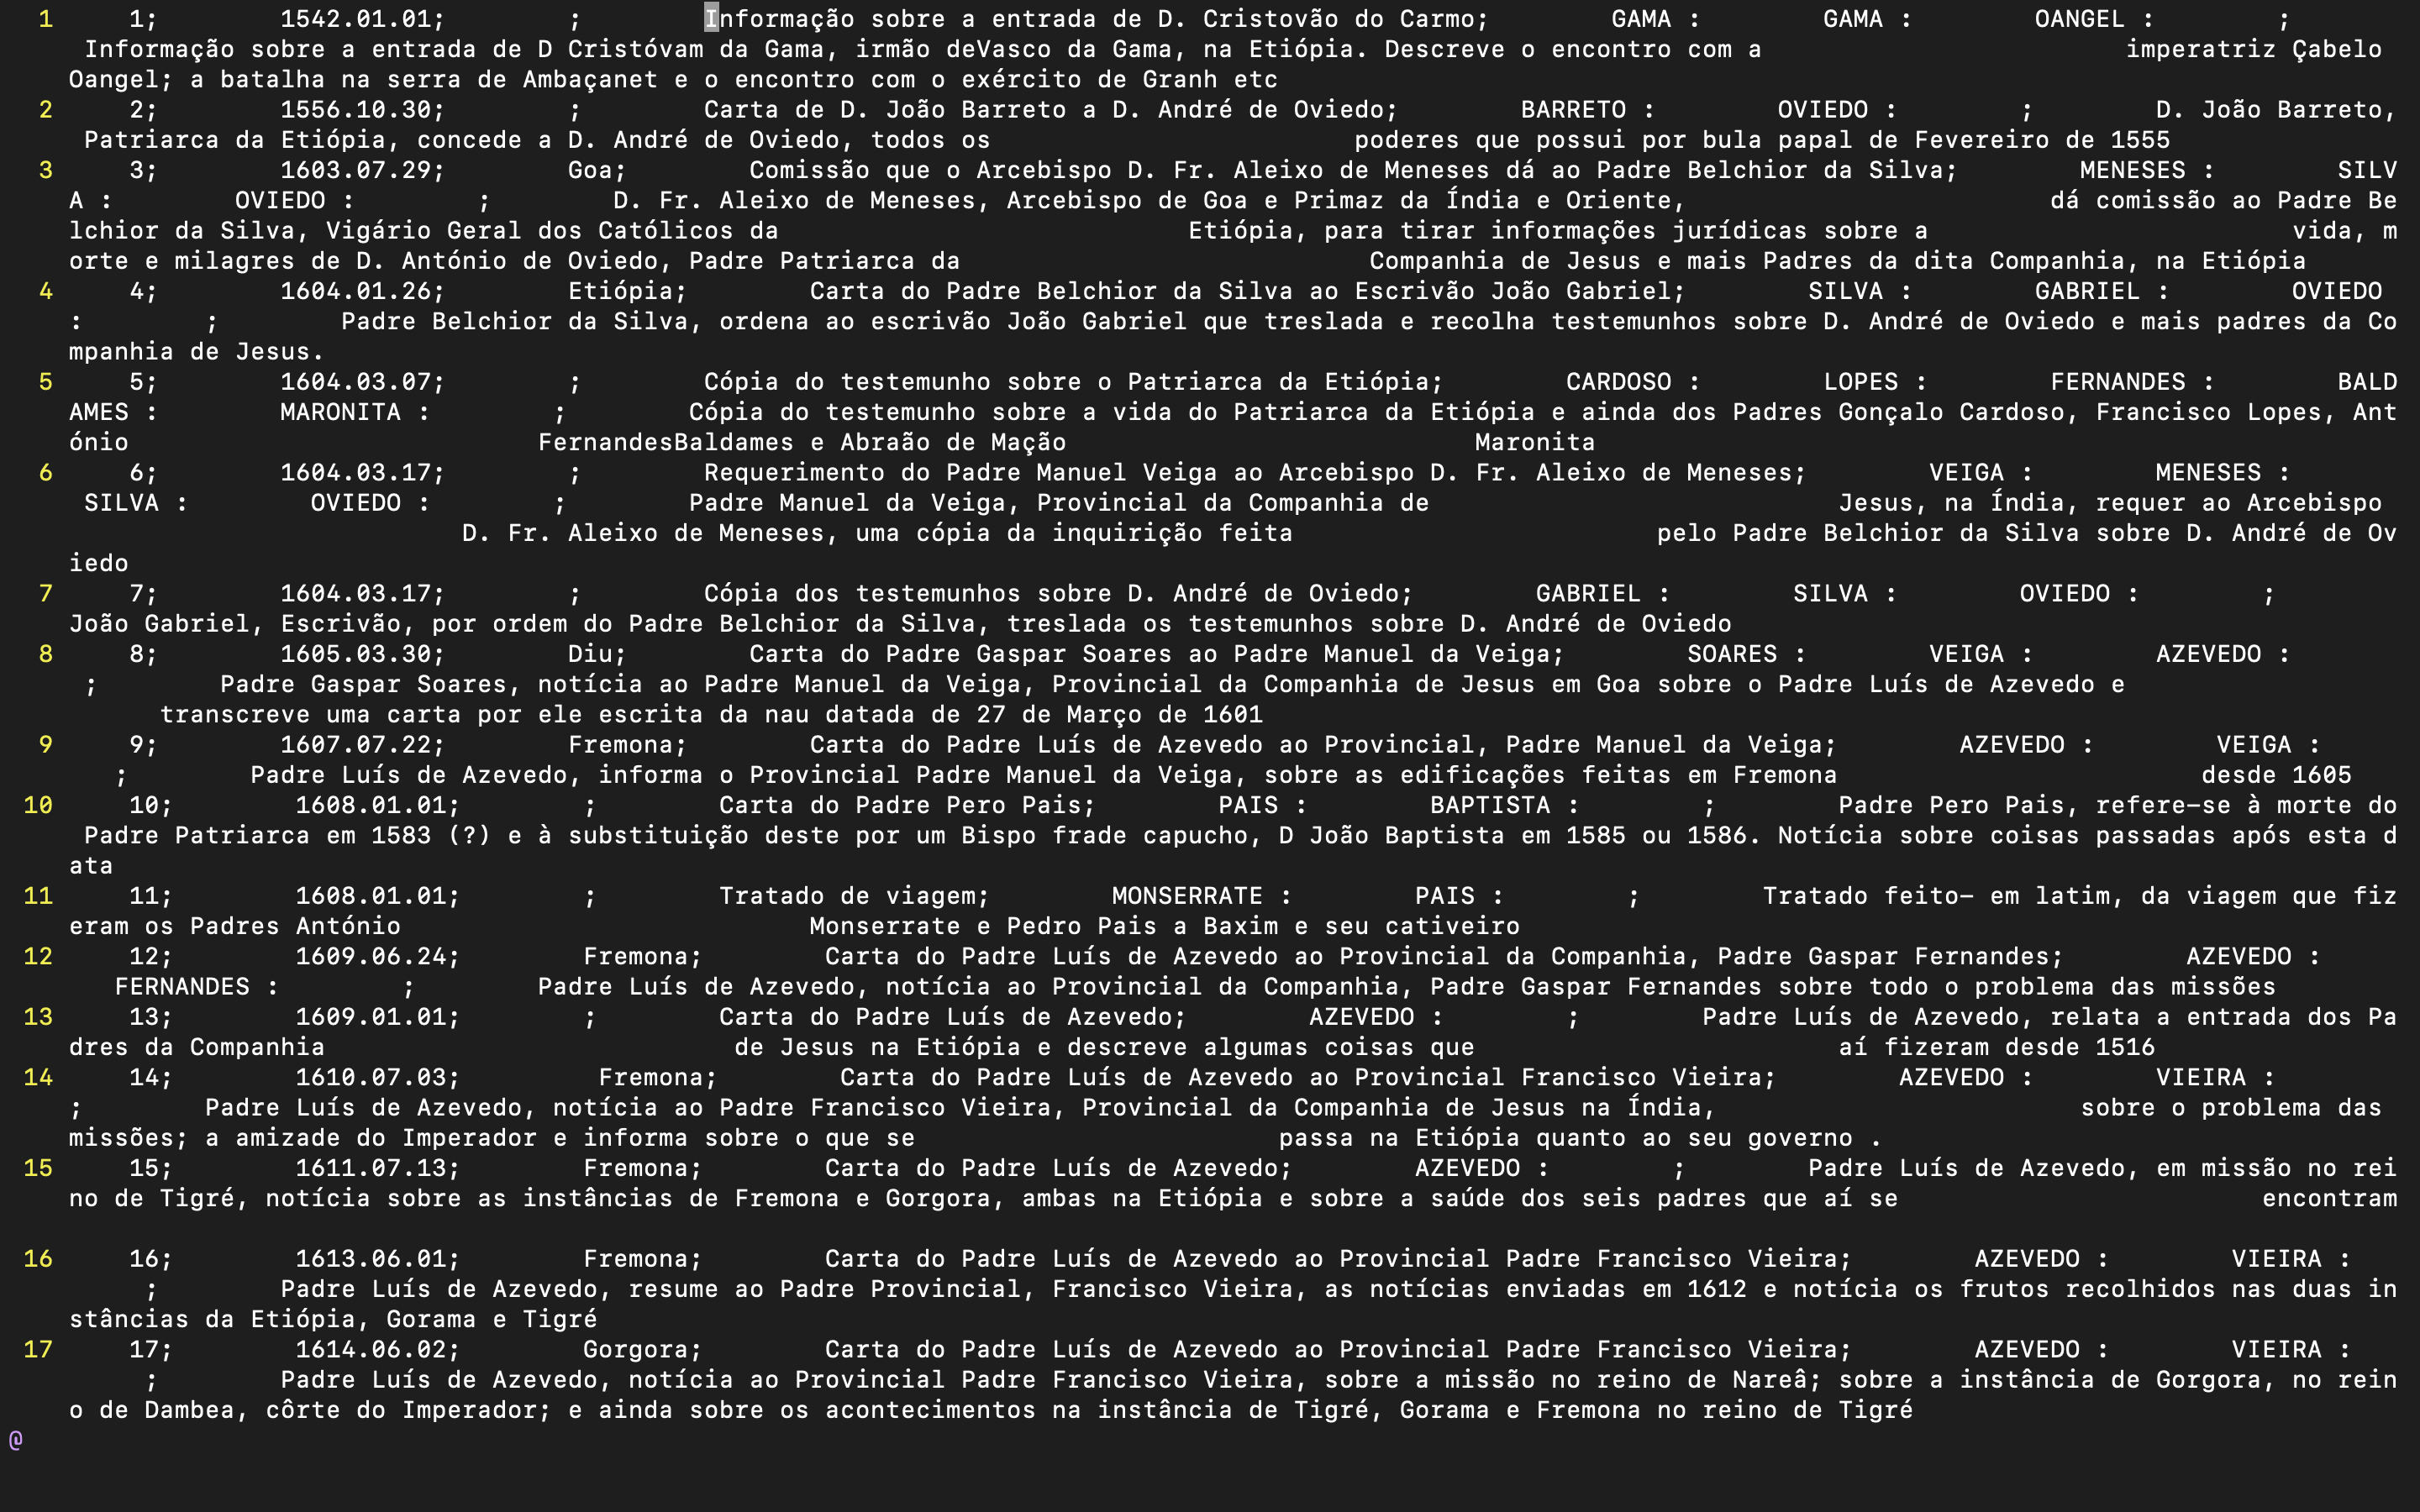
\includegraphics[width=\textwidth]{cartas2.png}
\caption{Ficheiro com os registos das cartas}
\end{figure}

\newpage
\section{Output's}

\quad De seguida, apresentámos excertos dos resultados obtidos após correr o comando:

\begin{verbatim}
    awk -f ex<n>.awk cartasetiopia.csv
        <n> := número do exercício
\end{verbatim}

\subsection{Número de cartas por local}
\begin{figure}[h]
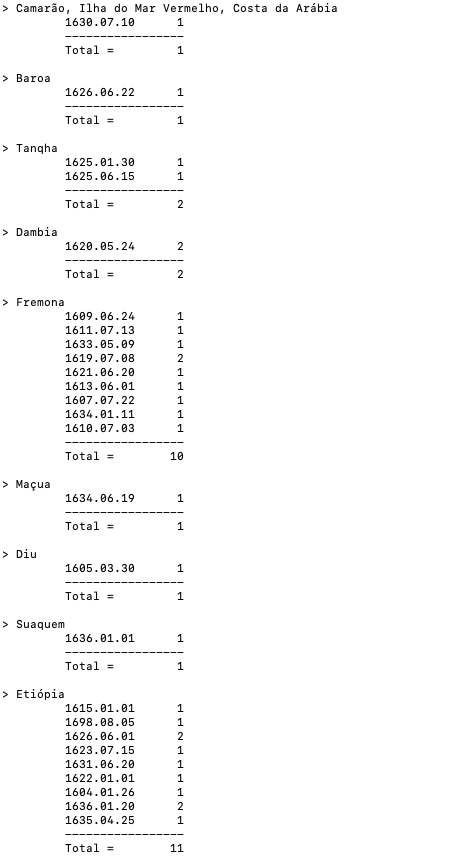
\includegraphics[scale=0.50]{ex1}
\caption{Resultado obtido no exercício 1}
\end{figure}

\subsection{Gerar Ficheiros HTML}
\begin{figure}[h]
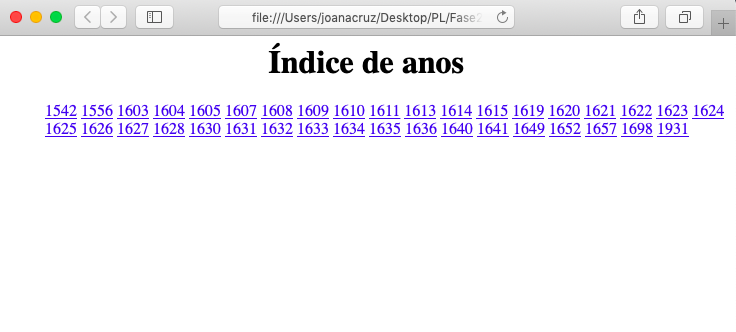
\includegraphics[scale=0.50]{ex21}
\caption{Resultado obtido no exercício 2 - HTML com índice dos anos das cartas}
\end{figure}

\begin{figure}[h]
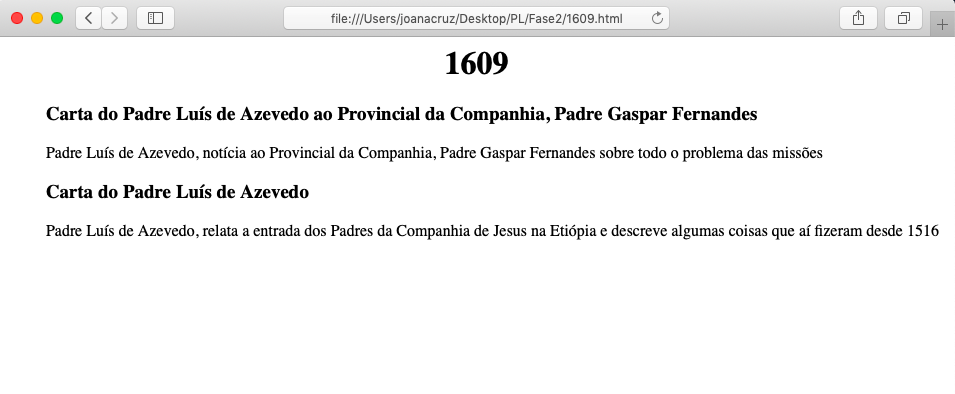
\includegraphics[width=\textwidth]{ex22}
\caption{Resultado obtido no exercício 2 - HTML correspondente a um ano}
\end{figure}

\newpage

\subsection{Lista de cartas}
\begin{figure}[h]
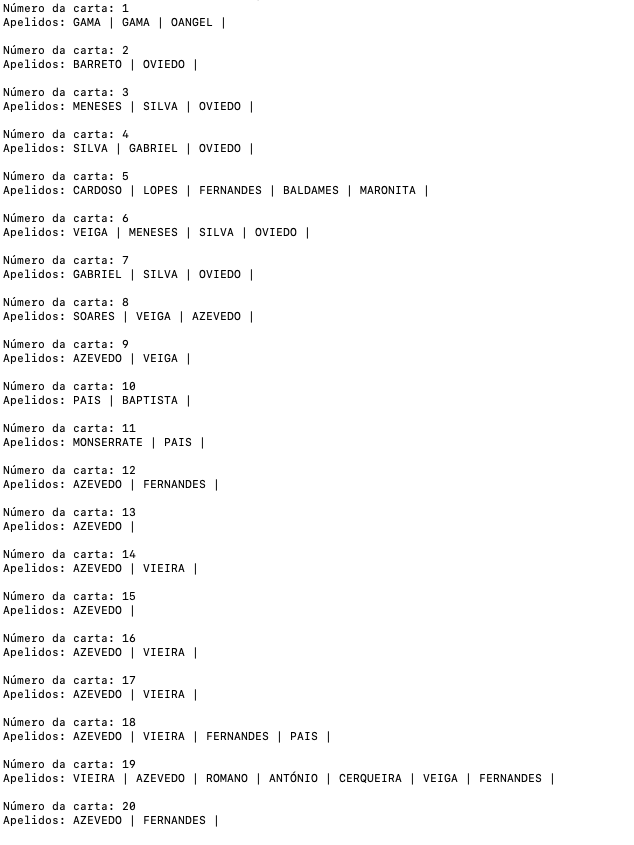
\includegraphics[scale=0.50]{ex3}
\caption{Resultado obtido no exercício 3}
\end{figure}

\newpage 

\subsection{Grafo DOT}
\begin{figure}[h]
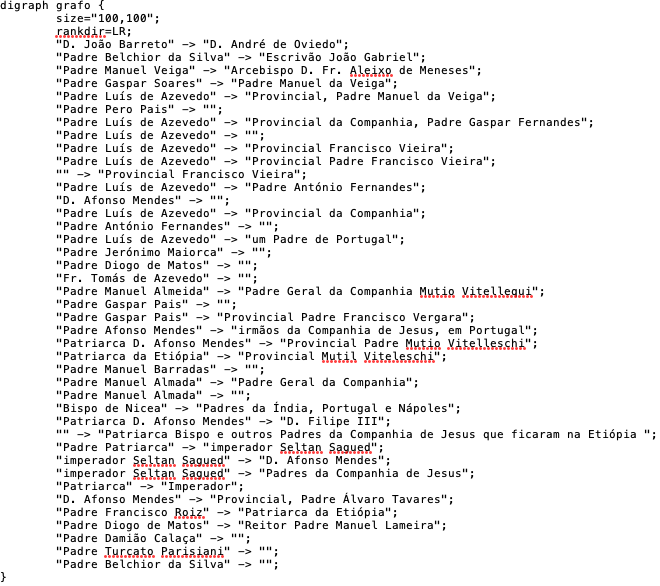
\includegraphics[width=\textwidth]{ex41}
\caption{Resultado obtido no exercício 4 - Ficheiro .gv}
\end{figure}

\begin{figure}[h]
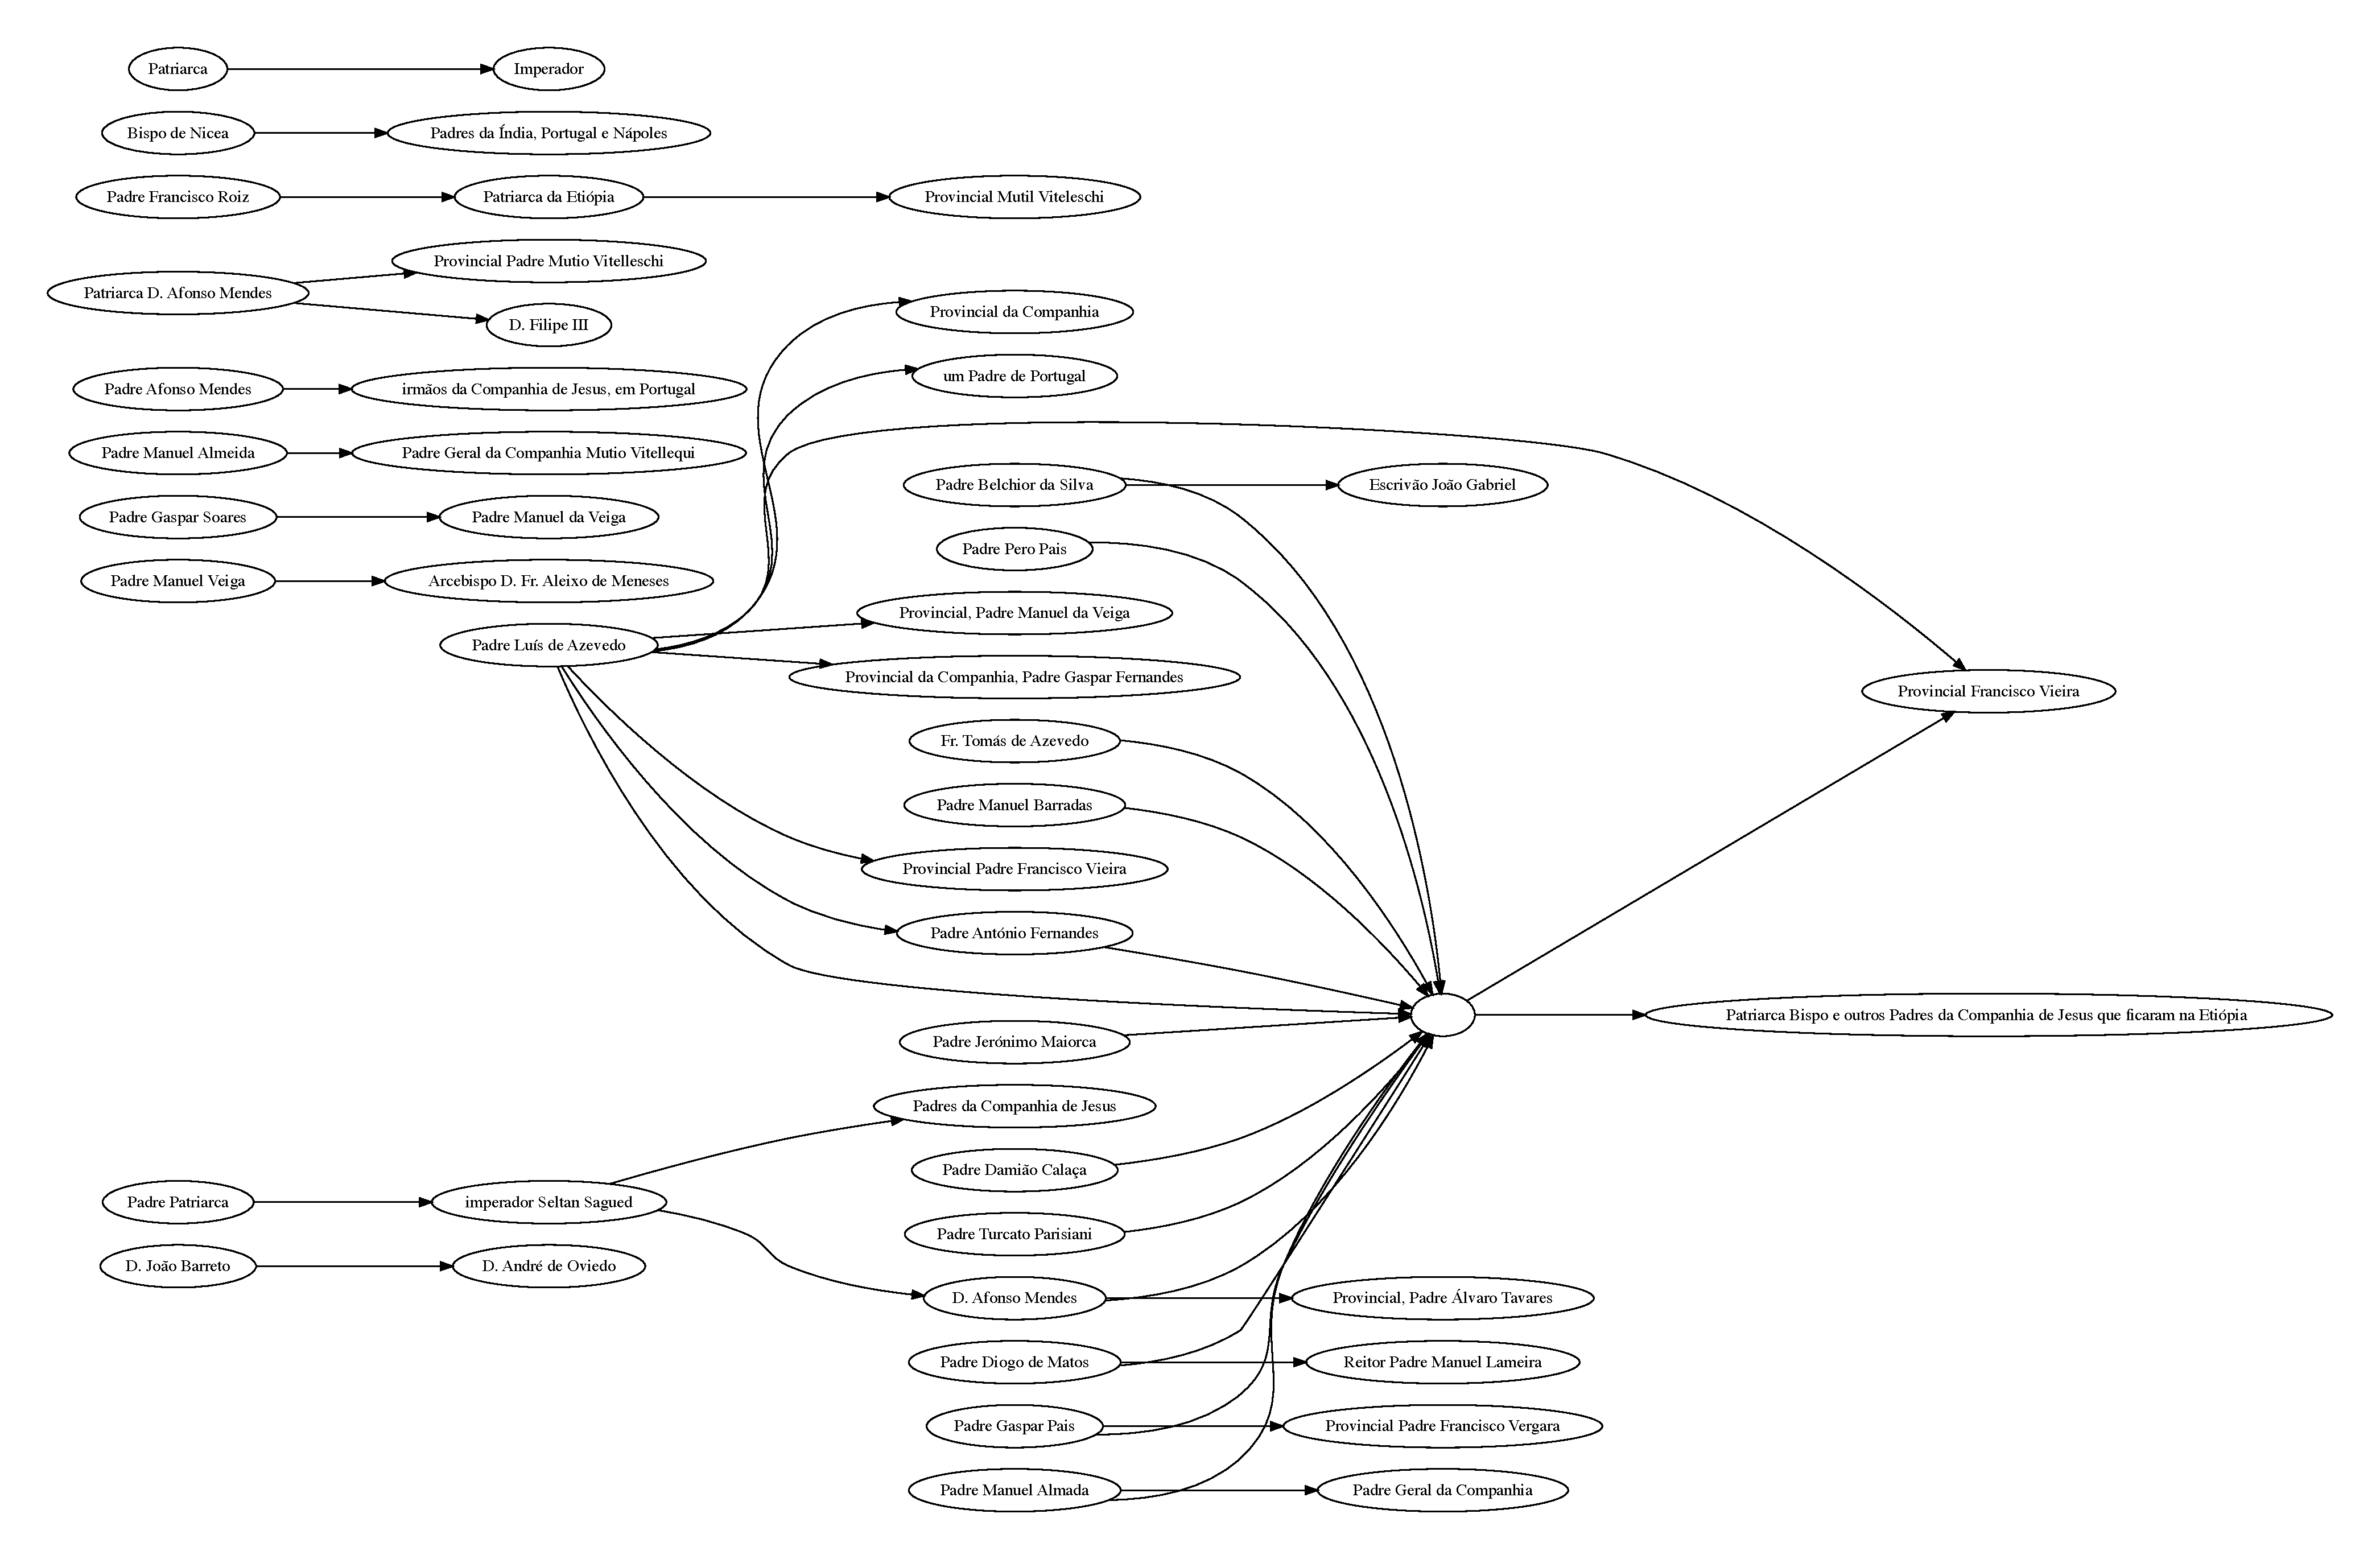
\includegraphics[scale=0.23]{grafo}
\caption{Resultado obtido no exercício 4 - Grafo obtido}
\end{figure}
\chapter{Conclusão}

\qquad A linguagem de programação \textbf{\textit{GAWK}} mostrou-se muito útil e versátil para resolver este tipo de trabalhos. Neste caso, uma vez que o ficheiro já estava com formato \textbf{\textit{CSV}}, o processo de filtrar e extrair informação de ficheiros tornou-se uma tarefa menos custosa, uma vez que o \textit{\textbf{GAWK}} apresenta vários mecanismos, intuitivos, de processar estes mesmos ficheiros.

\qquad As maiores dificuldades encontradas pelo grupo estão relacionadas com a normalização de dados, uma vez que tivemos que, através de expressões regulares, encontrar/filtrar os dados de forma totalmente genérica. 

\qquad Podemos concluir que o \textbf{\textit{GAWK}} é uma ferramenta muito poderosa e útil para manipular ficheiros/arquivos de dados de uma maneira simples e eficaz.

\end{document}
